%!TEX root = ../vernier.tex
\section{Colormap} \label{sec:colormap}
Colormaps are mapping functions that for every point of the domain of interest, assign to it a color based on the scalar value at that point. In this tool, three different color mapping schemes based on the ColorBrewer's \cite{ref:colorbrewer} samples were implemented. A sequential colormap was used to display the current normalized value of a chosen metric, a diverging colormap was used to show the increase/decrease of a given metric from revision $T_{n-1}$ to $T_{n}$, and a categorical colormap was used to group classes from the same package into a single color.

\begin{figure}[H]
  \centering
  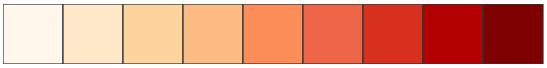
\includegraphics[width=0.6\textwidth]{figures/seq.png}
  \caption{Sequential Colormap}
  \label{fig:seq}
\end{figure}

\begin{figure}[H]
  \centering
  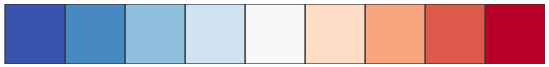
\includegraphics[width=0.6\textwidth]{figures/div.png}
  \caption{Diverging Colormap}
  \label{fig:div}
\end{figure}

\begin{figure}[H]
  \centering
  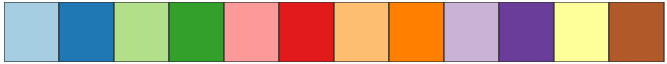
\includegraphics[width=0.6\textwidth,height=0.9cm]{figures/quali.png}
  \caption{Qualitative Colormap}
  \label{fig:quali}
\end{figure}
